\documentclass{article}

\usepackage[T2A]{fontenc}
\usepackage[utf8]{inputenc}
\usepackage[russian,english]{babel}
\usepackage{url}
\usepackage{tablefootnote}
\usepackage[left=2cm,right=2cm,top=2cm,bottom=2cm,bindingoffset=0cm]{geometry}
\usepackage[colorlinks=true,urlcolor=blue]{hyperref}
\usepackage[pdftex]{graphicx}

\newcommand*{\titleIG}{\begingroup
\centering
\vspace*{7\baselineskip}
\Huge
The VMware DVS plugin \\
for Fuel 6.1 installation guide \\
\vspace*{1.3\baselineskip}\hfill\today
\vfill
\pagenumbering{gobble}
\newpage
\pagenumbering{arabic}
\endgroup}

\begin{document}

\titleIG

\tableofcontents

\newpage

\section{Revision history}

\begin{table}[h]
\begin{tabular}{|p{4cm}|p{4cm}|p{4cm}|p{4cm}|}
\hline
Version & Revision date & Editor & Comment \\
\hline
0.1 & 09.01.2015 & Igor Gajsin & Created the first version.\\
 & & (igajsin@mirantis.com) & \\
\hline
\end{tabular}
\end{table}

\section{Document purpose}

The purpose of this document is to describe how to install, configure and use the VMware DVS plugin for Fuel 6.1.

\section{Key terms, acronyms and abberviations}

\begin{table}[h]
\begin{tabular}{|l|p{12cm}|}
\hline
\textbf{Term/acronym/abbreviation} & \textbf{Definition} \\
\hline
VM & Virtual Machine \\
\hline
MOS & Mirantis OpenStack \\
\hline
OVS & Open vSwitch \\
\hline
Neutron ML2 plugin & The Neutron Modular Layer 2 plugin is a framework allowing OpenStack Networking to simultaneously utilize the variety of layer 2 networking technologies \\
\hline
vmware\_dvs driver & The driver in the Neutron ML2 plugin which provides interaction with dvSwitch on vCenter \\
\hline
VMware DVS plugin & The plugin for Fuel which installs and configures vmware\_dvs driver on a MOS environment \\
\hline
dvSwitch & distributed vSwitch on VMware ESXi \tablefootnote{\url{http://kb.vmware.com/selfservice/microsites/search.do?language=en_US&cmd=displayKC&externalId=1010555}}\\
\hline
VMware ESXi & bare-metal hypervisor \\
\hline
VMware vCenter Server & Central control point for VMware vSphere \\
\hline
VMware vSphere & VMware's cloud computing virtualization operating system. \\
\hline
\end{tabular}
\end{table}

\section{The VMware DVS plugin}

MOS supports using vCenter as a hypervisor in a vCenter-only or heterogeneous, mixed with KVM environments. There is the vmware\_dvs  driver for Neutron ML2 plugin which provides usage Neutron for networking in such environments. Thereby environments receives an advanced network features:

\begin{itemize}

\item Ability to create multi-tier networks (e.g., web tier, db tier, app tier).

\item Control over IP addressing.

\item Ability to insert an configure their own services (e.g., firewall, IPS)

\item VPN/Bridge to remote physical hosting or customer premises.

\end{itemize}

\section{Licensing information}

\begin{table}[h]
\begin{tabular}{|p{8cm}|p{8cm}|}
\hline
\textbf{Component} & \textbf{License} \\
\hline
vmware\_dvs driver & Apache 2.0 \\
\hline
VMware DVS plugin & Apache 2.0 \\
\hline
\end{tabular}
\end{table}

\section{Assumptions and limitations}

\subsection{Assumptions}

\begin{enumerate}

\item dvSwitch must be provisioned by using vCenter firstly and manually.

\item There must be a mapping between physical network and dvSwitch:

\begin{enumerate}

\item different physnet to different dvSwitch \\ $($i.e.~physnet1:dvswitch1, physnet2:dvswitch2$)$,

\item different physnet to the same dvSwitch \\ $($i.e.~physnet1:dvswitch1, physnet2:dvswitch1$)$.

\end{enumerate}

\item VLANs will be used as a tenant network separation by KVM’s OVS and ESXi’s
     dvSwitch (must be the same for tenant network regardless which switch type OVS
     or dvSwitch)

\item There must be an ability to:

\begin{enumerate}

\item create / terminate a port group on dvSwitch

\item bind port from such port group to a VM

\item disable state of the neutron port group or port on dvSwitch

\item assign multiple vNIC to a single VM deployed on ESXi

\end{enumerate}

\item Name of driver is vmware\_dvs

\item Plugin supports addition controller-nodes after deploy.

\item Plugin has to carry with it code of vmware\_dvs and all their dependencies to be independent from network’s conditionals when install.

\end{enumerate}

\subsection{Limitations}

\begin{itemize}

\item VMware DVS plugin be enabled only in environments with Neutron as the networking option.

\item Only VLANs are supported for tenant network separation (VxLAN support can be added later, if project will be continued).

\item Only vSphere 5.5 is supported

\end{itemize}

\section{Requirements}

The plugin has the following requirements for software

\begin{table}[h]
\begin{tabular}{|p{8cm}|p{8cm}|}
\hline
\textbf{Requirements} & \textbf{Version} \\ \hline
Fuel & 6.1 \\ \hline
vCenter & 5.5 \\ \hline
\end{tabular}
\end{table}

\section{Installation Guide}

\subsection{Prerequisites}

This guide assumes that you have installed Fuel and all the nodes of your future environment are discovered and functional. Note, that you need to have a connectivity to correctly configured vCenter with precreated dvSwitch and clusters.

\subsection{Obtaining the VMware DVS plugin}

You can download it from \href{https://www.mirantis.com/products/openstack-drivers-and-plugins/fuel-plugins/}{Fuel Plugins Catalog} or build from the \href{https://github.com/stackforge/fuel-plugin-vmware-dvs}{github repositories} via some steps:

\begin{enumerate}

\item Create and activate a virtual environment:

{\tt
\$ virtualenv fpb \\\$ . fpb/bin/activate
}

\item Install the fuel plugin builder:

{\tt
$($fpb$)$user@host:/path\$ pip install fuel-plugin-builder
}

\item Get plugin sources from github.

{\tt $($fpb$)$user@host:/path\$ git clone https://github.com/stackforge/fuel-plugin-vmware-dvs.git}

\item Patch the template file in the fuel plugin builder

{\tt
$($fpb$)$user@host:/path\$ patch  fpb/lib/python2.7/site-packages/fuel\_plugin\_builder/ \\
                /templates/build/plugin\_rpm.spec.mako fuel-plugin-vmware-dvs/hack.diff
}

\item Build the plugin

{\tt $($fpb$)$user@host:/path\$ fpb \textemdash\textemdash build fuel-plugin-vmware-dvs/ \\
Plugin is built}

\item Put the plugin into Fuel Master node

{\tt
\$ scp fuel-plugin-vmware-dvs-1.0-1.0.1-1.noarch.rpm <Fuel Master node ip>:/tmp
}

\item Login to the Fuel Master node and install the plugin:

{\tt
\$ ssh root@<Fuel Master node ip>

[root@nailgun \~]\# fuel plugins \textemdash\textemdash install /tmp/fuel-plugin-vmware-dvs-1.0\-1.0.1\-1.noarch.rpm

[root@nailgun ~]\# fuel plugins \\
DEPRECATION WARNING: /etc/fuel/client/config.yaml exists and will be used as the source for settings. This behavior is deprecated. Please specify the path to your custom settings file in the FUELCLIENT\_CUSTOM\_SETTINGS environment variable.\\

\begin{tabular}{l|l|l|l}
id & name                   & version & package\_version\\
\hline
2  & fuel-plugin-vmware-dvs & 1.0.1   &2.0.0          \\
\end{tabular}
}

\end{enumerate}

\subsection{Removing the VMware DVS plugin}

To uninstall Zabbix plugin, follow these steps:

\begin{enumerate}

\item Delete all Environments in which VMware DVS plugin has been enabled.

\item Uninstall the plugin:\\
{\tt
\# fuel plugins \textemdash\textemdash remove fuel-plugin-vmware-dvs==1.0.1
}

\item Check if the plugin was uninstalled successfully:

\begin{tabular}{l|l|l|l}
id & name                   & version & package\_version\\
\hline
  &  &   &          \\
\end{tabular}

\end{enumerate}

\newpage

\section{Configuring VMware DVS plugin}

\begin{enumerate}

\item \href{https://docs.mirantis.com/openstack/fuel/fuel-6.1/user-guide.html#create-a-new-openstack-environment}{Create a new OpenStack environment} with Fuel UI wizard

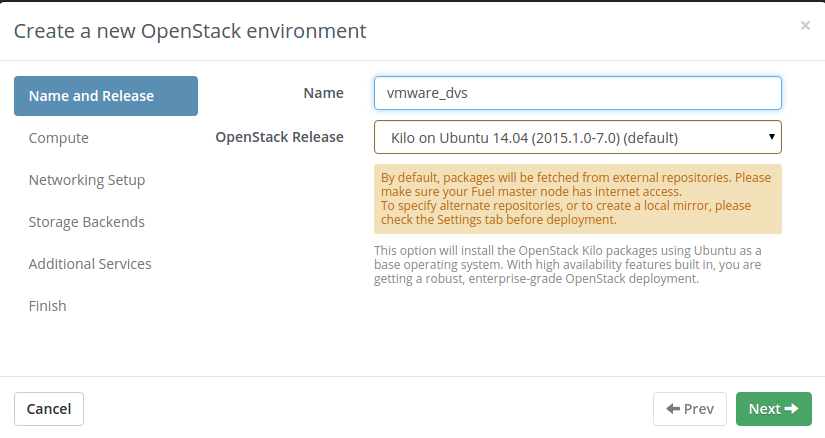
\includegraphics[scale=0.8]{pics/create}

\item Please set vCenter checkbox on choosing compute's type step.

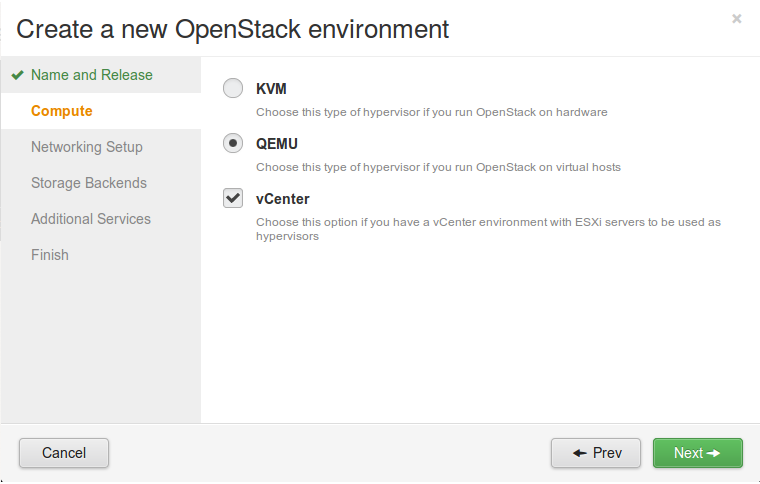
\includegraphics[scale=0.8]{pics/compute}

\newpage

\item Please select Neutron with VLAN segmentation network model, which is the only network type supported with VMware DVS plugin

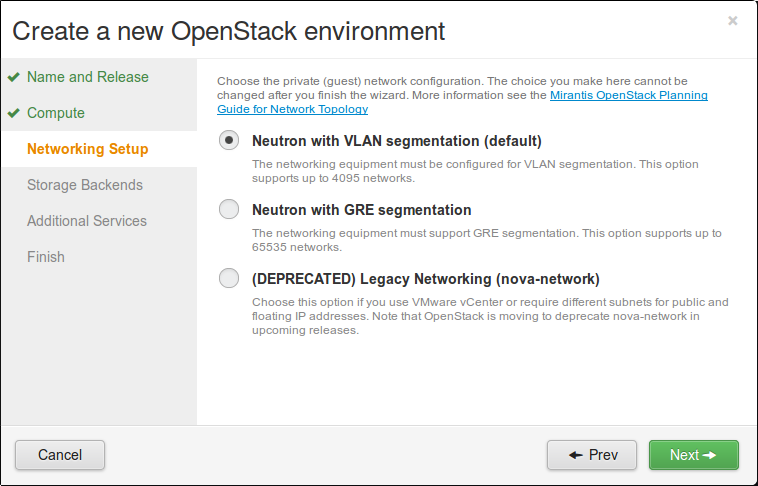
\includegraphics[scale=0.8]{pics/net}

\item There are no limitations on other steps in the wizard.

\item Add at least 1 Controller and 1 Compute node to the environment.

\item Turn on the plugin usage checkbox and set correct name of dvSwitch in the Settings tab.

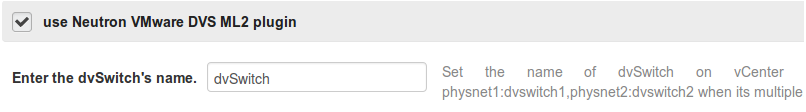
\includegraphics[scale=0.8]{pics/settings}

\newpage

\item Fill the vmware configuration fields on the VMware tab.

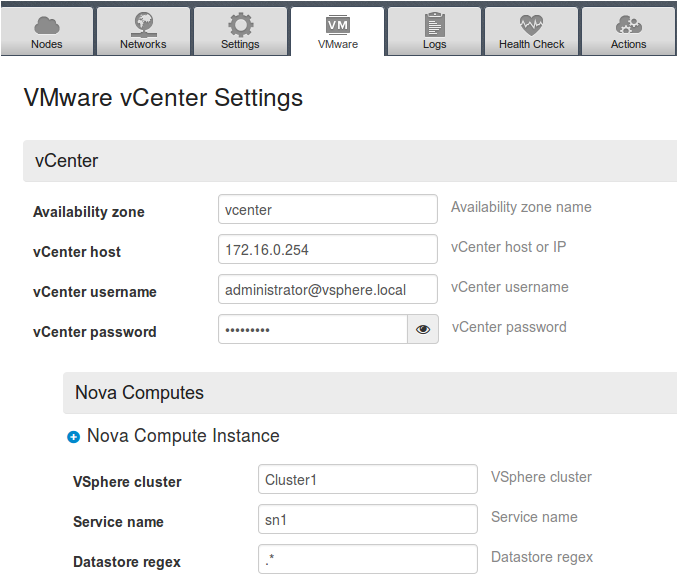
\includegraphics[scale=0.75]{pics/vmware}

The rest configuration is up to you. See \href{https://docs.mirantis.com/openstack/fuel/fuel-6.1/user-guide.html}{Mirantis OpenStack User Guide} for instructions to configure other options.

\item Click ``Deploy changes'' to deploy the environment.

\end{enumerate}

\section{Usage Guide}

Once OpenStack has been deployed, we can start using Neutron for networking. The net04 port group should appear on the vCenter:

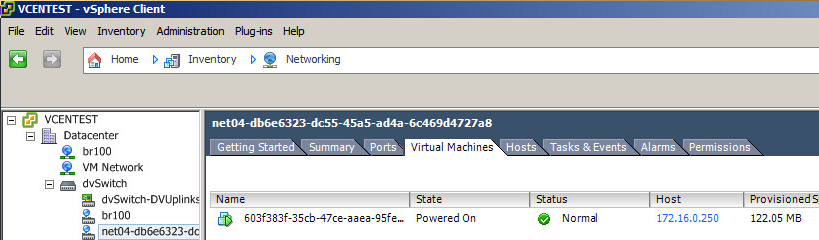
\includegraphics[scale=0.8]{pics/net04pg}

\newpage

Network topology on Horizon should looks like:

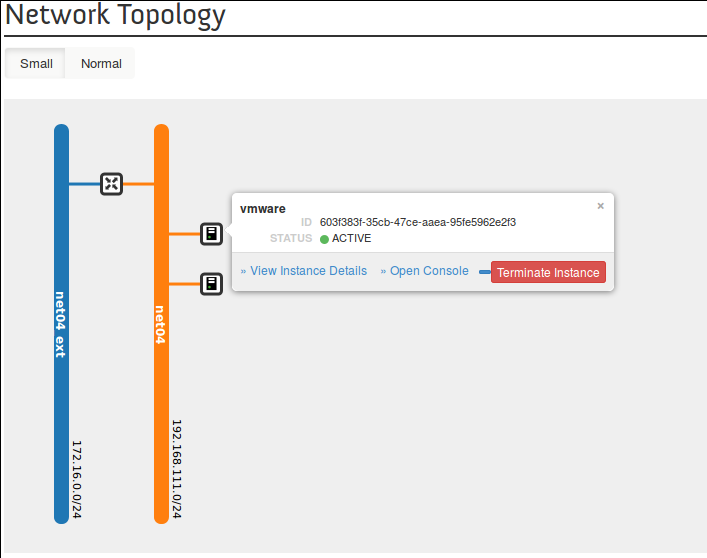
\includegraphics[scale=0.8]{pics/topology}

where vmware is an instace located on the vCenter.

You can use Neutron for such instance totally same way as for KVM located instances.

\end{document}
